\section{Introducción}

\subsection{Motivación del trabajo}

La movilidad urbana eficiente constituye uno de los principales desafíos para las ciudades contemporáneas, especialmente en un contexto de creciente demanda de sostenibilidad, aumento del parque automovilístico y limitaciones estructurales de las infraestructuras viarias existentes. Una gestión adecuada del tráfico no solo repercute positivamente en la calidad de vida de la ciudadanía, sino que también tiene un impacto directo en la reducción del consumo energético, la mejora de la seguridad vial y la disminución de la contaminación atmosférica.

En este escenario, la predicción del tráfico emerge como una herramienta clave para anticiparse a situaciones de congestión, disrupciones u otros eventos que puedan comprometer la fluidez de la circulación. Gracias al avance de la inteligencia artificial y, en particular, del aprendizaje profundo, hoy es posible desarrollar modelos que integren datos en tiempo real y capturen patrones complejos mediante el uso de arquitecturas sofisticadas.

El creciente interés por aplicar estos avances en entornos reales de alta densidad urbana motiva la realización del presente trabajo, que se centra en el desarrollo de un modelo de predicción de tráfico con enfoque local en la provincia de Bizkaia, uno de los territorios más dinámicos y problemáticos desde el punto de vista de la movilidad en el norte de España.

\subsection{Planteamiento del problema}

La provincia de Bizkaia presenta un conjunto de particularidades que complican la gestión efectiva del tráfico. Su orografía abrupta limita la expansión de nuevas vías y condiciona la distribución del tráfico en corredores específicos, donde la saturación es frecuente. A esto se suma la alta densidad poblacional, especialmente en el área metropolitana de Bilbao, y una variabilidad meteorológica significativa, que puede afectar las condiciones de circulación de forma impredecible.

\begin{figure}[h]
	\centering
	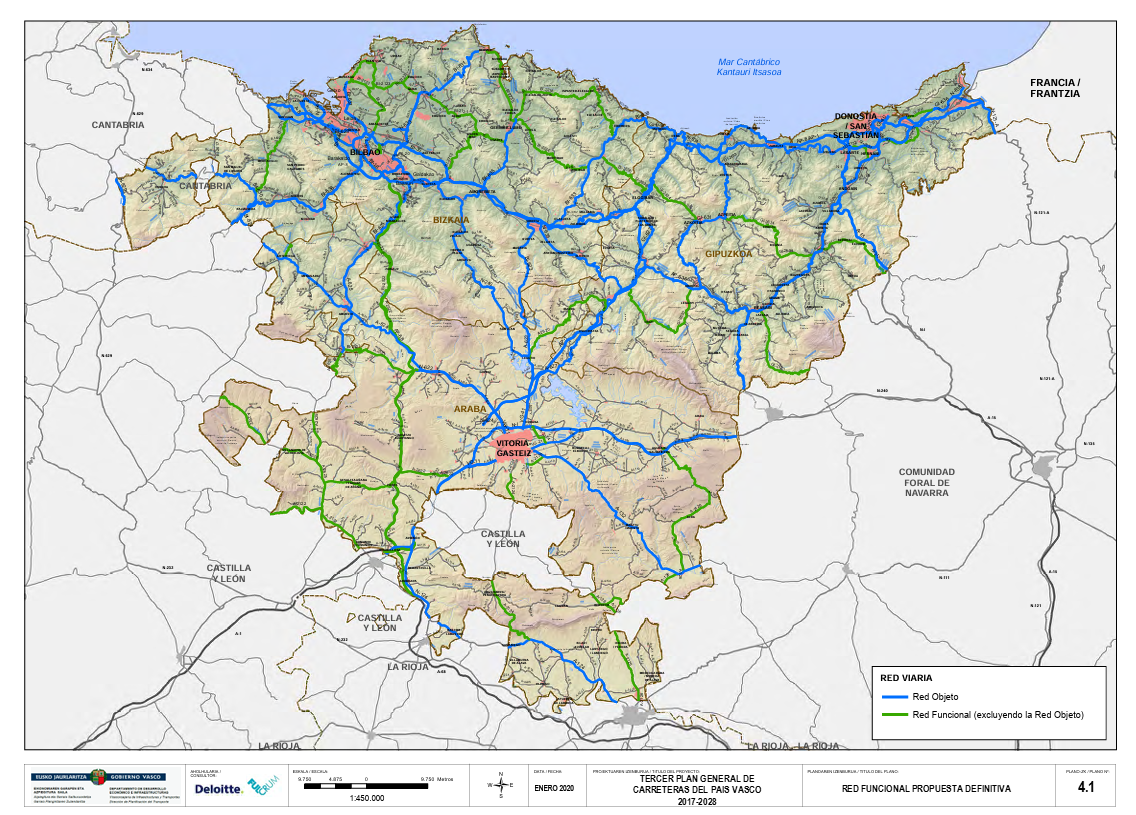
\includegraphics[scale=0.5]{includes/red_viaria_capv.png}
	\caption[Red viaria de la CAPV, extraído del Tercer Plan General de Carreteras del País Vasco 2017-2028. Fuente: https://www.euskadi.eus/tercer-plan-general-de-carreteras-del-pais-vasco-2017-2028/web01-a2bideko/es/]{Red viaria de la CAPV}
	\label{fig:red_viaria}
\end{figure}


En la figura \ref{fig:red_viaria} se aprecia la complejidad de la red viaria en la \acrshort{capv}. En diversas zonas como los accesos a Bilbao, los túneles del Kadagua o los enlaces con la A-8, se producen episodios de congestión recurrentes, especialmente en horas punta y durante condiciones meteorológicas adversas. Aunque Bizkaia dispone de una infraestructura \acrshort{its} notable (sensores, cámaras, estaciones meteorológicas), no se cuenta aún con herramientas predictivas suficientemente precisas que permitan anticipar estos episodios y facilitar la toma de decisiones en tiempo real.

La complejidad inherente a los datos de tráfico, caracterizados por correlaciones espacio-temporales, no linealidades y gran volumen, exige modelos capaces de capturar dichas relaciones con eficacia. Las aproximaciones tradicionales, basadas en regresión o aprendizaje automático clásico, resultan insuficientes en este contexto. Se necesita un enfoque moderno, capaz de integrar múltiples fuentes de datos y aprender representaciones complejas.

En respuesta a los retos mencionados, este trabajo propone el diseño, desarrollo y evaluación de un modelo de predicción del tráfico en Bizkaia basado en redes neuronales con arquitectura Transformer. Esta arquitectura ha demostrado un rendimiento sobresaliente en tareas de modelado secuencial y captura de dependencias a largo plazo, gracias a su mecanismo de atención, lo que la convierte en una candidata idónea para abordar la predicción de tráfico con alta precisión.

El modelo se alimentará de datos abiertos sobre tráfico y meteorología, publicados por organismos como Open Data Euskadi y Euskalmet, lo que garantiza la transparencia, replicabilidad y aplicabilidad del sistema propuesto. A través de un enfoque empírico, se evaluará la eficacia del modelo frente a enfoques tradicionales, utilizando métricas estándar y se estudiará su potencial para integrarse en sistemas actuales de gestión del tráfico.

Este documento se estructura de la siguiente manera: el capítulo 2 presenta una revisión del estado del arte, analizando los principales trabajos relacionados y su aplicabilidad al contexto de Bizkaia; el capítulo 3 define los objetivos del trabajo y la metodología seguida; los capítulos siguientes abordarán el desarrollo del proyecto y conclusiones finales, aunque esto es un trabajo por determinar.

\subsection{Introducción general del trabajo}

\vspace*{\fill}
\selectlanguage{spanish}
\begin{abstract}
	La predicción precisa del tráfico es clave para optimizar la movilidad y el uso de infraestructuras, especialmente en la \acrlong{capv} y más en concreto en la provincia de Bizkaia, donde la orografía, densidad urbana y condiciones meteorológicas suponen retos añadidos. Sin embargo, la complejidad inherente a los datos de tráfico, caracterizados por fuertes correlaciones espacio-temporales y patrones no lineales, dificulta su modelado y predicción exacta. Este trabajo propone un modelo de predicción basado en redes neuronales con arquitectura Transformer, capaz de capturar dependencias espacio-temporales complejas mediante mecanismos de atención que asignan pesos dinámicos a segmentos relevantes. Se emplearán datos abiertos de tráfico y meteorología procedentes de la provincia de Bizkaia. La validación se realizará con datos reales y se comparará frente a modelos tradicionales de redes neuronales, demostrando mejoras significativas en precisión. El sistema resultante ofrece una herramienta robusta y eficiente para la gestión del tráfico en tiempo real, con potencial para anticipar congestiones y optimizar la toma de decisiones operativas.
\end{abstract}
\textbf{Palabras clave}: Predicción del tráfico, Aprendizaje profundo, Transformers, Redes neuronales, Correlación espacio-temporal, Datos abiertos, Comunidad Autónoma del País Vasco, Bizkaia

\vfill

\selectlanguage{english}

\begin{abstract}
	Accurate traffic forecasting is essential for optimising mobility and infrastructure usage, especially in the Autonomous Community of the Basque Country (\acrshort{capv}) and particularly in the province of Bizkaia, where the region’s orography, urban density, and weather variability present additional challenges. However, the inherent complexity of traffic data, characterised by strong spatio-temporal correlations and non-linear patterns, makes its modelling and prediction difficult. This work proposes a prediction model based on neural networks with Transformer architecture, capable of capturing complex spatio-temporal dependencies through attention mechanisms that dynamically assign weights to relevant segments. Bizkaia's open traffic and weather datasets will be used. The model will be validated with real-world data and compared against traditional neural network models. The outcome will be a robust and efficient tool for real-time traffic management, with the potential to anticipate congestion and support the optimisation of operational decision-making.
\end{abstract}

\textbf{Keywords}: Traffic forecasting, Deep learning, Transformers, Neural networks, Spatio-temporal correlation, Open data, Autonomous Community of the Basque Country, Bizkaia
\selectlanguage{spanish}
\vspace*{\fill}